\documentclass[conference]{IEEEtran}

\usepackage[pdftex]{graphicx}
\graphicspath{ {./images/} }

\usepackage{amsmath}
\usepackage{amsfonts}
\usepackage{amssymb}
\interdisplaylinepenalty=2500

\usepackage{array}

\begin{document}
\title{Multicarrier Modulation: Carrier Frequency Offset}
\author{\IEEEauthorblockN{Daryl Leon Wasden, Ph.D.}
\IEEEauthorblockA{Salt Lake City, Utah\\
Email: dwasden@outlook.com\\
Prepared for Signal Laboratories, Inc.}}

\maketitle

\begin{abstract}
A simulation-based study was carried out to quantify the performance of several
multicarrier modulation (MCM) techniques, namely discrete multitone (DMT) also
called orthogonal frequency division multiplexing (OFDM), filtered multitone (FMT)
and staggered multitone (SMT) also sometimes called OFDM-OQAM. Simulations were
made to compare the performance of these three MCM techniques with regards to
carrier frequency offset (CFO). For now, the additive white Gaussian noise (AWGN)
channel is considered. It is of particular interest to our group what will happen
to the beam-forming capability of multiple radios as they combine at a receiver
with slightly different frequency offsets. For this reason, we present results
for a point-to-point link, and then we present results where two radios are 
transmitting to a single user and report the expected loss due to CFO.
% Eventually put results here.
\end{abstract}

\section{Introduction}
\label{sec:intro}

This document provides simulation results that will help characterize the various
multicarrier modulation (MCM) techniques in the presence of carrier freqeuency
offset (CFO). MCM techniques are known to be more sensitive to CFO than single
carrier modulation techniques. Three MCM techniques are considered in this paper.
One is discrete multitone (DMT) also known as orthogonal frequency division
multiplexing (OFDM). Another one is filtered multitone (FMT), and the last one
is staggered multitone also sometimes called OFDM-OQAM. The latter two techniques
belong to the general class called filter bank multicarrier (FBMC). % \cite{farhang2009}.

DMT is a technique that has garnered much attention in the commercial, governmental,
and academic communities. It has been well-studied and is included in our analysis
to provide a baseline for comparing the other techniques. The flavor of DMT considered
here uses a cyclic prefix to allow easy and efficient equalization for each subcarrier
signal.

FMT is a technique that does not allow subcarrier bands to overlap. This means that
each subcarrier has the maximum isolation possible from its environment. This results
in excellent out-of-band rejection and robustness to CFO. Because subcarrier bands are
not allowed to overlap, an FMT system with the same number of subcarriers as a DMT or 
SMT system requires more bandwidth. Equivalently, given the same total bandwidth and
subcarrier spacing, FMT will populate the band with a fewer number of subcarriers.

SMT is a technique that allows the subcarrier bands to overlap, but time-staggers
the in-phase and quadrature streams so that they are transmitted at time intervals
that are half a symbol period apart. This staggering allows the signal to be 
decoded at the receiver with the ISI term remaining orthogonal on each subcarrier.
SMT uses overlapping subcarriers and does not require a cyclic prefix. For this
reason, it may be argued to have the highest potential for spectrum efficiency
of the three techniques considered here.

This document is organized in the following manner. Section~\ref{sec:MCM} 
describes the three multicarrier modulation techniques that were simulated:
DMT, FMT, and SMT. Section~\ref{sec:Models} describes the two different
channel models that were considered: the point-to-point model and the
beamforming model. Section~\ref{sec:Methods} describes the simulations
and how the systems were modeled in simulation. Section~\ref{sec:Results}
reports on the results of the simulations. Finally, a conclusion is 
provided in Section~\ref{sec:Conclusion}.

Mathematical conventions used in this work. Continuous-time signals are
represented as functions of a continuous-valued time variable $t$ (for
example, $x(t)$, $y(t)$, and $z(t)$). Discrete-time signals are represented
as functions of a discrete (integer-valued) variable $n$ (for example, 
$x[n]$, $y[n]$, and $z[n]$). The convolution operator (for both continuous
and discrete time) is denoted with the $*$ symbol (for example, $x(t) * y(t)$).
A vector is denoted in lowercase with a bold font (for example, $\mathbf{x}$, 
$\mathbf{y}$, and $\mathbf{z}$). A matrix is denoted in uppercase with a bold
font (for example $\mathbf{A}$, $\mathbf{B}$, and $\mathbf{C}$). When we want
to talk about the distribution of something we will use the symbol $\sim$ which
can be read ``is distributed as'' when read aloud. Two common distributions are
the normal (Gaussian) distribution which is denoted $N(\mu, \sigma^2)$ where
$\mu$ is the mean and $\sigma$ is the standard deviation and the uniform 
distribution which is denoted $U(\alpha, \beta)$ where the elements are
enumerated using the real numbers (for continuous distributions) or the 
integers (for discrete distributions). The symbol $\alpha$ represents the 
leftmost (least) element possible and $\beta$ is the rightmost (greatest) 
element. It should be clear from context whether the distribution is a
continuous distribution or a discrete distribution.

\section{Multicarrier Modulations}
\label{sec:MCM}

This section provides details on the MCM techniques that are compared in the
simulations. First, we provide a framework for the discussion of MCM in general.
This is a framework that applies equally well to DMT, FMT, and SMT. Following
this, a general description of each technique is provided. Each technique
corresponds to setting the framework parameters in a specific way. The
parameter choices for each MCM technique is described in each subsection.

MCM modulation takes a fast serial data stream and divides it into multiple
parallel data streams. This allows many of the computations to be run at 
slower rates in parallel when compared to the single carrier data stream
at the same rate. MCM also eases the task of equalization, eliminating the 
need for lengthy equalization at the receiver before decoding. These advantages
have lead to the adoption of MCM techniques in many broadband modems. %\cite{80211, 80216, LTE, DSL}

\begin{figure*}[ht!]
	\centering
	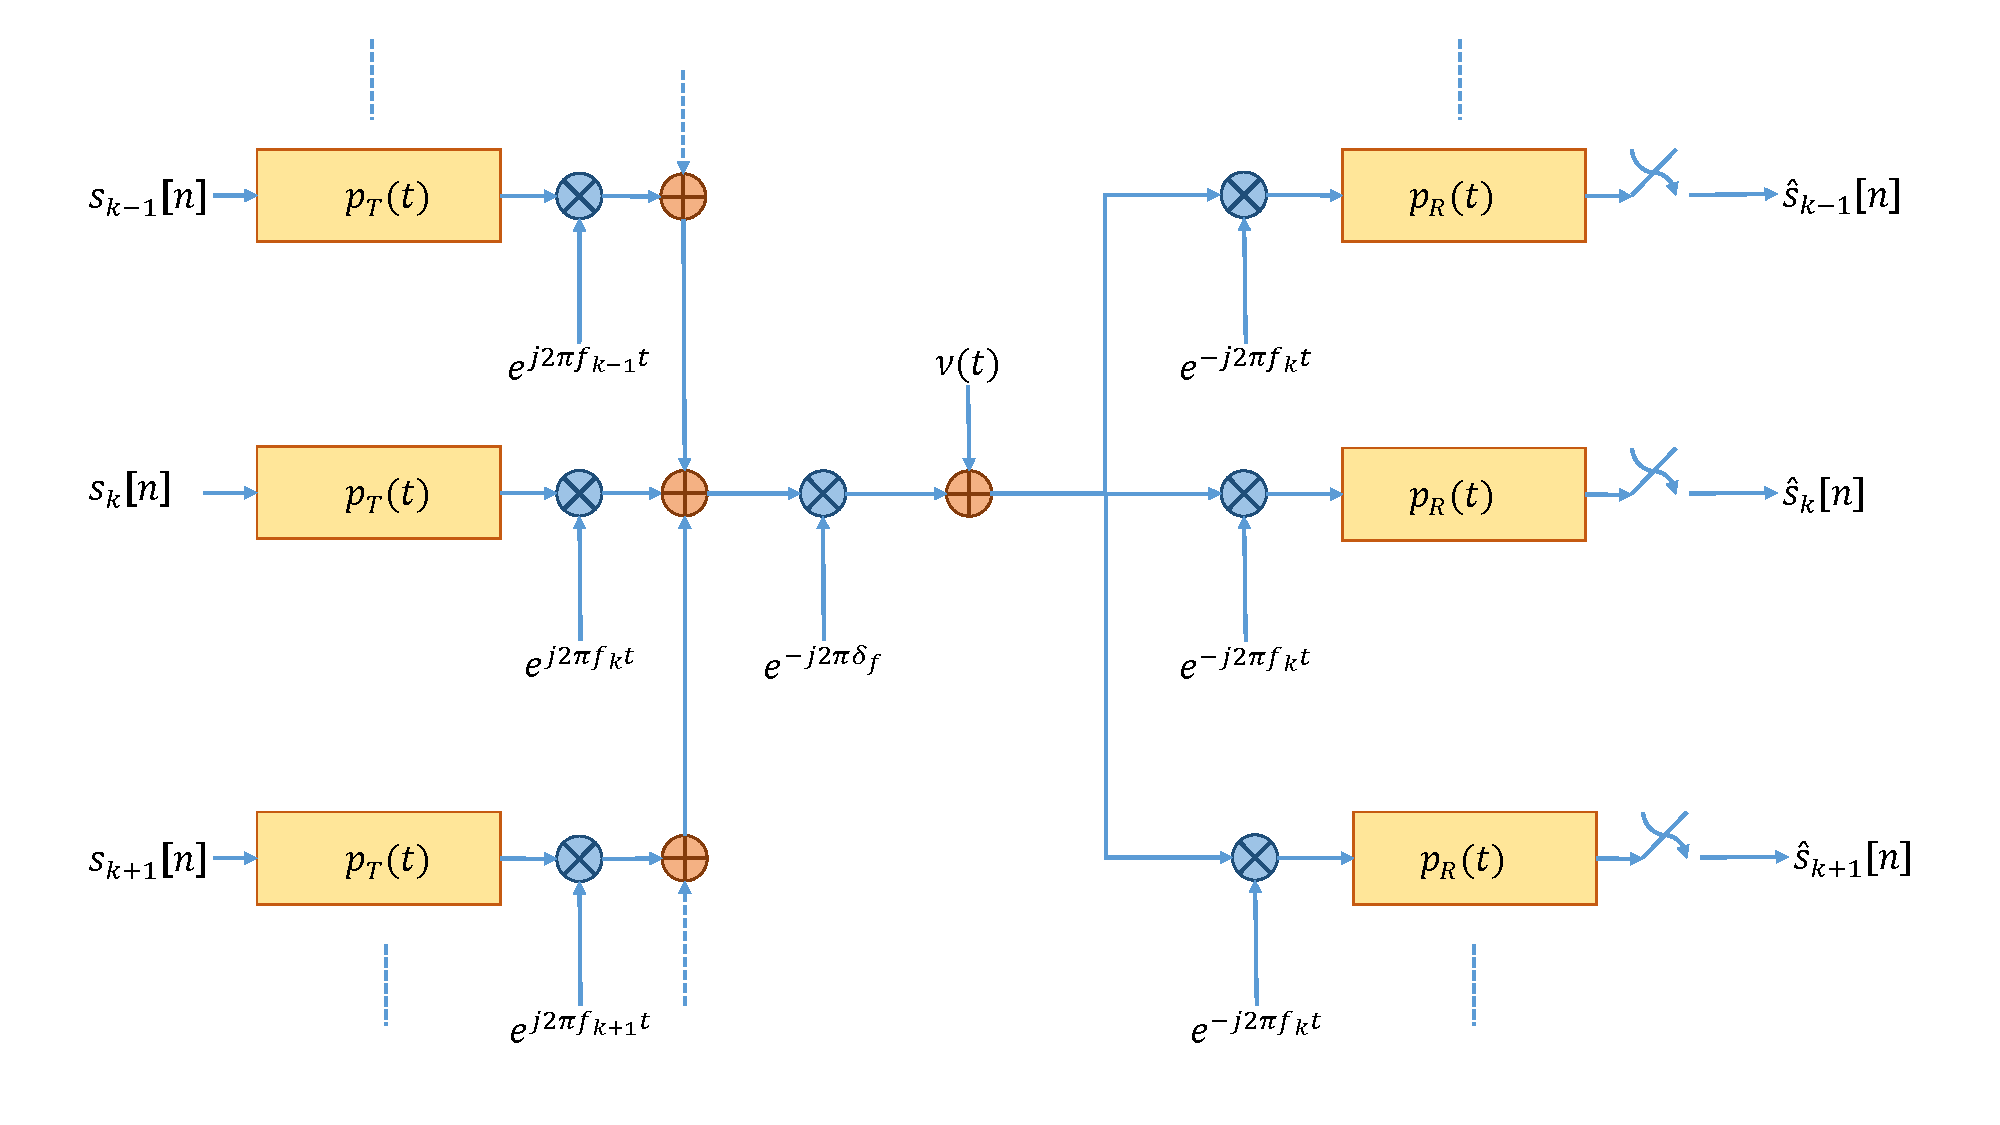
\includegraphics[scale=0.5]{MCM_pic.pdf}
	\caption{Block diagram showing details for the MCM model we use.}
	\label{fig:mcm_model}
\end{figure*}

Figure~\ref{fig:mcm_model} shows the layout of our simulation model. The
parameters of the model relevant to the different MCM techniques are the
choice of the transmit pulse shaping filter $\p_T(t)$, the choice of the 
receive matched filter $\p_R(t)$, and the choice of subcarrier frequencies 
$f_0, f_1, ...$. These three parameters can be adjusted to yield DMT, FMT,
and SMT systems.

Also shown in Figure~\ref{fig:mcm_model} are the two imperfections we will 
consider: the CFO, $\delta_f$, and the additive white gaussian noise (AWGN),
$\nu(t)$. These will be addressed in Section~\ref{sec:Models}.

\subsection{Discrete Multitone (DMT)}

DMT uses a rectangular pulse shape at the transmitter that is longer than the
receiver matched filter in such a way that the receiver timing can be offset
and still be ``matched'' to a portion of the transmit signal. 

\subsection{Filtered Multitone (FMT)}

\subsection{Staggered Multitone (SMT)}

\section{Channel Models}
\label{sec:Models}

\subsection{Point-to-Point}
\subsection{Beamforming}

\section{Simulation Methods}
\label{sec:Methods}

\subsection{Point-to-Point}
\subsection{Beamforming}

\section{Simulation Results}
\label{sec:Results}

\subsection{Point-to-Point}
\subsection{Beamforming}

\section{Conclusion}
\label{sec:Conclusion}

\end{document}
